\documentclass{scrartcl}
\usepackage[utf8]{inputenc}
\usepackage{pgf-pie}
\usepackage{subfigure}
\usepackage{hyperref}
\usepackage{cite}
\usepackage{amsmath}
\usepackage{amssymb}
\usepackage{graphicx}
%\documentclass{book}
\renewcommand\thesubsection{\Alph{subsection}}


%opening
\title{Assignment 1}
\author{Daan Spijkers, s1011382\\ Tomás Catalán López, s1081589\\ Willem Lambooy, s1009584}

\begin{document}
\maketitle

\textbf{Note: you can find the GitHub repository at}
\url{github.com/dspijkers/nacu}.

\section*{Exercise 1}
Schemata A1 has more wildcards than A2: $o(A1) < o(A2)$. Since both schemata have the same amount of bits, the chance of a non-wildcard bit flipping in A1 is less than the chance of that happening in A2.

Mathematically, this can be computed as follows (with $p_m=0.01$):
\begin{itemize}
 \item Probability of a bit not being flipped after mutation: $1-p_m=0.99$.
 \item Probability that A1 survives: $S_m(A1)=(1-p_m)^{o(A1)}=0.99^4\approx0.961$.
 \item Probability that A2 survives: $S_m(A2)=(1-p_m)^{o(A2)}=0.99^5\approx0.951$.
\end{itemize}

\section*{Exercise 2}
Any problem that for example requires a specific combination of bits, that also has no variance in the fitness of the population would make the BBH not hold, for example:\\
\begin{center}
$\displaystyle f(x_1,x_2,x_3)=\mathrm{ \{ }
_{0 \; if \; not}
^{1\;if \; (x_1,x_2,x_3)=(0,0,1)))}$
\end{center}

\section*{Exercise 3}
\begin{itemize}
\item[(a)]

For the roulette wheel selection we calculate the probabilities of choosing an individual $x$ like this: $P(x) = f(x)/\sum_{x}f$
\newline
The results for $f(x)$ are in Table \ref{table:table2_1_1} and Figure \ref{fig:pie2_1_1}. The results for $f_1(x)$ are in Table \ref{table:table2_1_2} and Figure \ref{fig:pie2_1_2}


\begin{table}[h!]
\centering
\begin{tabular}{| c | c | c |}
\hline
$x$ & $f(x)$ & $P(x)$ \\
\hline
2 & 4 & $4/29 = 0.14$ \\
\hline
3 & 9 & $9/29 = 0.31$ \\
\hline
4 & 16 & $16/29 = 0.55$ \\
\hline
$Total$ & 29 & 1 \\
\hline
\end{tabular}
\caption{Results for $f(x)$}
\label{table:table2_1_1}
\end{table}

\begin{figure}[h!]
\centering

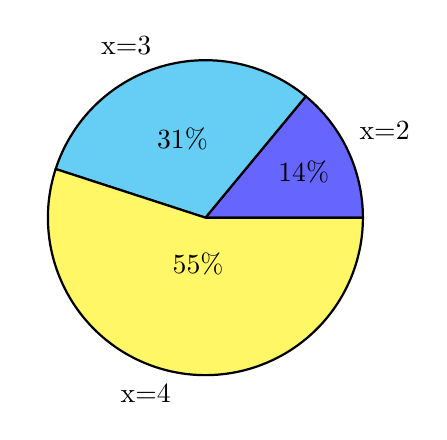
\begin{tikzpicture}

\pie[radius=2]{14/x=2,
    31/x=3,
    55/x=4}

\end{tikzpicture}
\caption{Pie chart for $f(x)$}
\label{fig:pie2_1_1}
\end{figure}

\begin{table}[h!]
\centering
\begin{tabular}{| c | c | c |}
 \hline
 $x$ & $f_1(x)$ & $P(x)$ \\
 \hline
 2 & 24 & $24/89 = 0.27$ \\
 \hline
 3 & 29 & $29/89 = 0.33$ \\
 \hline
 4 & 36 & $36/89 = 0.4$ \\
 \hline
 $Total$ & 89 & 1 \\
\hline
\end{tabular}
\caption{Results for $f_1(x)$}
\label{table:table2_1_2}
\end{table}

\begin{figure}[h!]
    \centering
    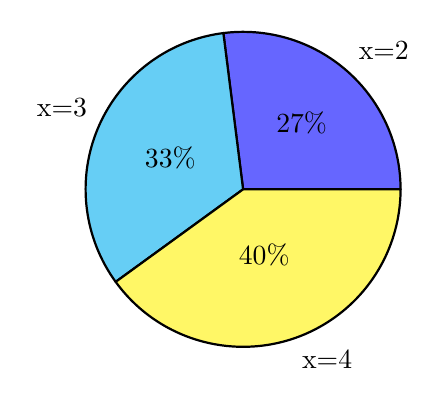
\begin{tikzpicture}

    \pie[radius=2]{27/x=2,
        33/x=3,
        40/x=4}

    \end{tikzpicture}
    \caption{Pie chart for $f_1(x)$}
    \label{fig:pie2_1_2}
\end{figure}

\item[(b)]
The function $f_1$ has low selection pressure, because the probabilities for each individual are quite similar. The function $f(x)$ on the other hand applies more pressure, giving more priority to $x=4$.
\item[(c)]
We can see that for scaled fitness, we have more equal probabilities for the individuals. Maybe we could use this in our favour, if we scale the fitness in the early stages of our algorithm, we would have more variability, and then we could narrow progressively the fitness to strengthen the selection pressure.

\end{itemize}

\section*{Exercise 4}
We have explained in more detail this exercise in the notebook (in the git
repository), but the results are in Figures \ref{a}, \ref{b} and \ref{c}:

\begin{figure}[!ht]
    \centering
    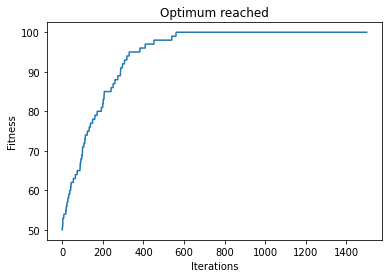
\includegraphics[width=0.65\textwidth]{4/output_a.png}
    \caption{Results of 4.a)}
    \label{a}
\end{figure}
\begin{figure}[!ht]
    \centering
    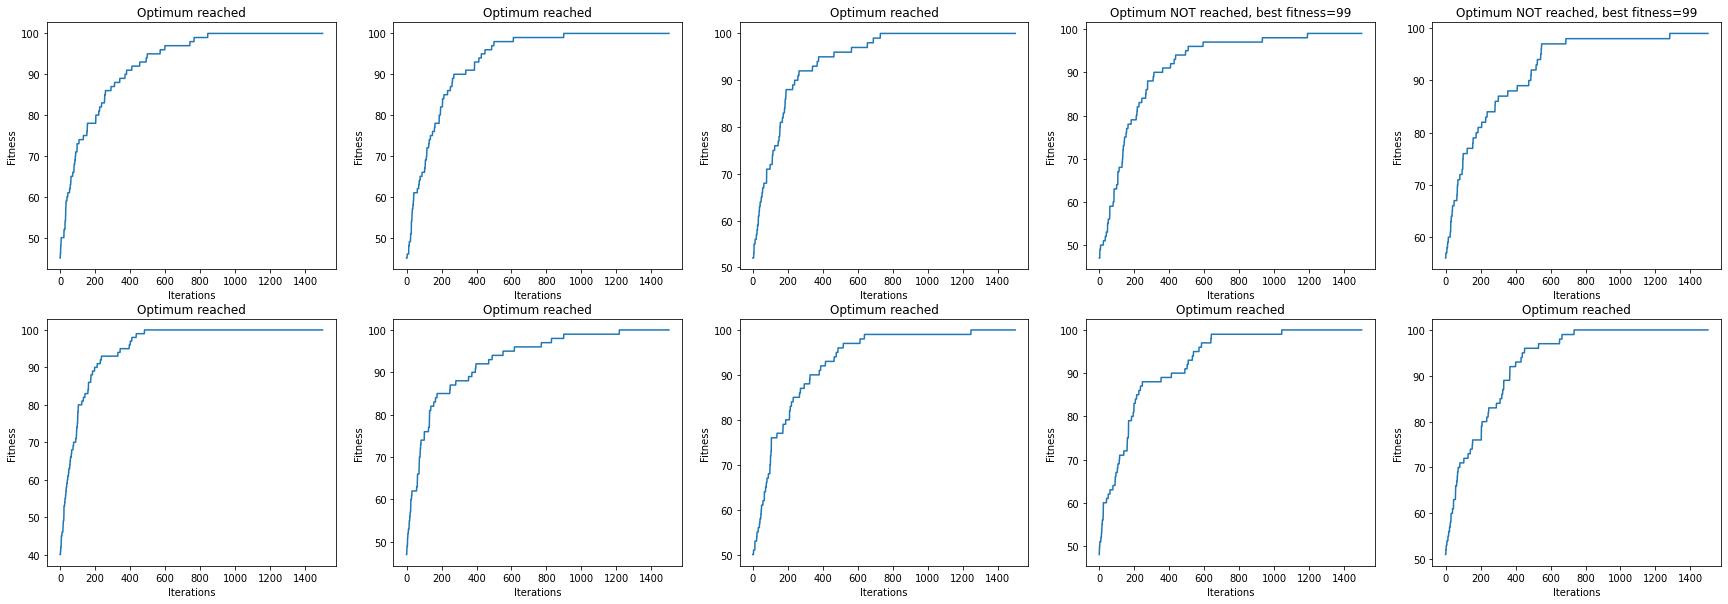
\includegraphics[width=\textwidth]{4/output_b.png}
    \caption{Results of 4.b)}
    \label{b}
\end{figure}
\begin{figure}[!ht]
    \centering
    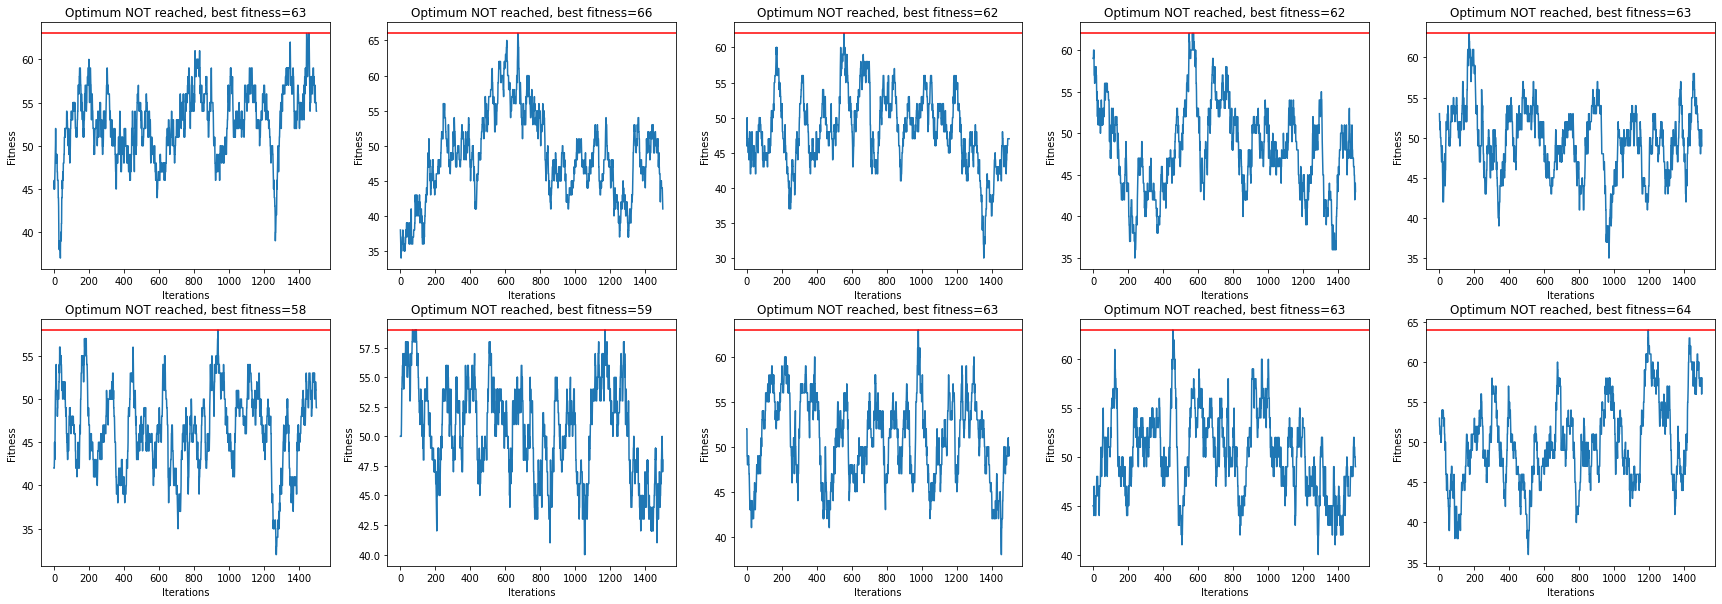
\includegraphics[width=\textwidth]{4/output_c.png}
    \caption{Results of 4.c)}
    \label{c}

\end{figure}

\section*{Exercise 5}
\begin{itemize}
 \item[(a)]
When we use a (1+5) ES, we consider a greater number of possible offspring in each iteration. Hence, compared to an (1+1) ES, it has a greater chance to produce better offspring in each iteration. A (1+1) ES tries one `path', and if it's better than the parent, will continue that way. One advantage that a (1+5) ES has is that as it explores more such paths, giving it a higher probability to make a bigger improvement.

 \item[(b)]
If $\lambda $ is equal to the number of possibilities at each step, we could say that a (1+$\lambda$) ES is the same as a greedy algorithm, because it would be making the best greedy choice at each step. If $\lambda$ is smaller, it cannot be guaranteed that it was a greedy algorithm.
\end{itemize}

\section*{6}
\begin{itemize}
 \item[(a), (b), (c)] The normal EA and the MA variant have been implemented in Python from scratch. The resulting program can be found in \texttt{6/TSPSolver.py}. Running the program results in four graphs being shown, these can also be seen in Figure \ref{fig:6}.

 Due to the high run-time complexity of the MA variant, the 2opt calls have been made multi-threaded. Changing parameters like the amount of cores to use or the (fixed) population size can be most easily done by changing the default parameters to the TSPSolver class.

 \emph{NOTE:} The 2opt algorithm was originally implemented in the MA in with the \texttt{repeat until no improvement is made} loop. This generated very boring output in the context of EA: the curve almost instantly goes down to the optimal solution, making the iterative and evolutionary aspects of the algorithm seem obsolete. Figure \ref{fig:6a} shows the output of this MA implementation. We opted to reduce the run-time complexity by removing this loop, thereby leaving more room for iterative improvement. The output of this MA implementation can be seen in Figure \ref{fig:6}. It should be noted that the former implementation produces better results, with all 10 runs amounting to the same optimal candidate. The latter implementation had different results each run, all a bit worse than the runs of the former.

 \item[(d)] You can see that the MA reaches a (seemingly) optimal solution much faster than the EA, which steadily decreases over the iterations.

 \item[(e)] No. The MA took ages longer to run, which already invalidates the comparison. MA finds a solution it does not improve on after just a few iterations, and these solutions are often (miles) better than what EA comes up with after 1500 generations. If you would let EA run for as long as it takes MA to run these 1500 generations, EA would run tens of thousands of iterations or perhaps much more even. After this amount of iterations it is likely that EA would approach or even surpass the result of MA.

 \item[(f)] In a paper by Liu, Huang and Zhong, titled ``Surrogate-assisted Multi-tasking Memetic Algorithm'' (\textbf{DOI:} 10.1109/CEC.2018.8477830), the state that existing solutions for their problem are designed based on basic evolutionary algorithm, and that the efficiency of such algorithm is not high enough on complicated optimisation problems. We hence draw the conclusion that while EA performs well on basic problems, it is sometimes not good enough when the problem gets more complicated. In these cases, hybridisation allows to optimise candidates, making a fitter population. A consideration should be made: increased running time of the MA on one side, versus requiring less iterations to find an optimal solution candidate on the other.
\end{itemize}

\begin{figure}
\centering
 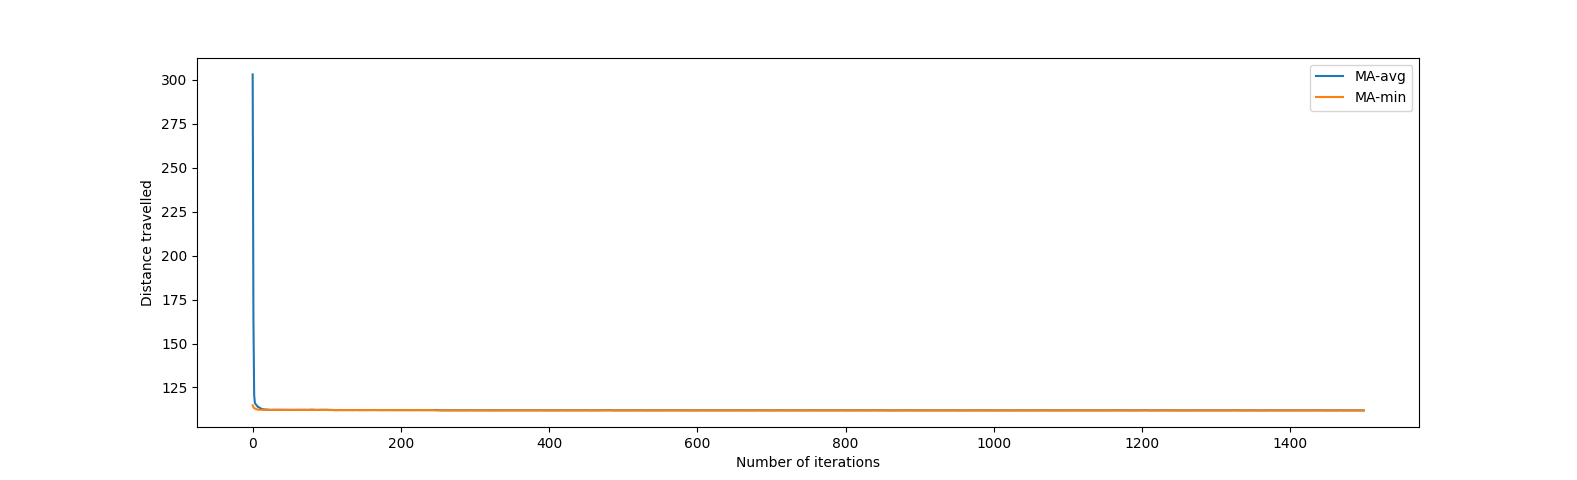
\includegraphics[width=\textwidth]{6/origMA2}

 \caption{Output of the original MA implementation. It consistently found an optimal distance of 112 for the TSP in \texttt{file-tsp.txt}, which is the best solution that was found by any algorithm made for this exercise.\label{fig:6a}}
\end{figure}


\begin{figure}[ht!]

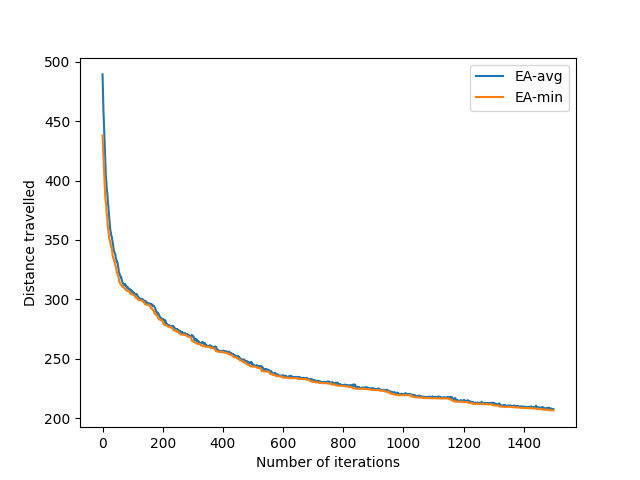
\includegraphics[width=0.5\textwidth]{6/6bEA}
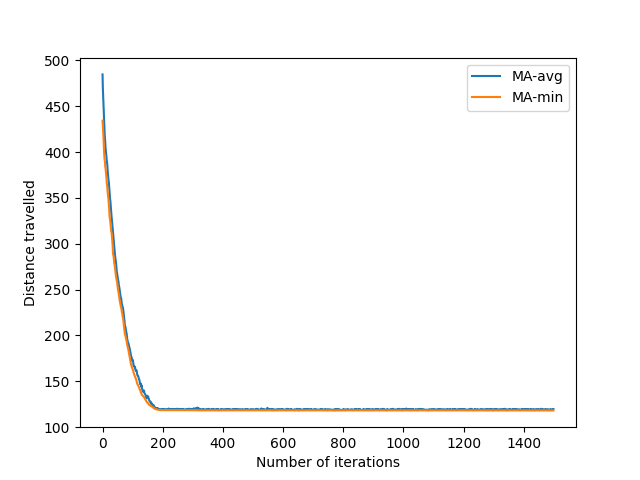
\includegraphics[width=0.5\textwidth]{6/6bMA}
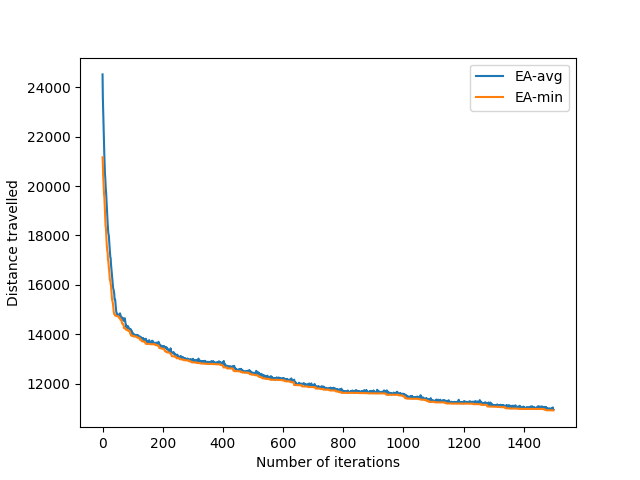
\includegraphics[width=0.5\textwidth]{6/6bEA_SYM}
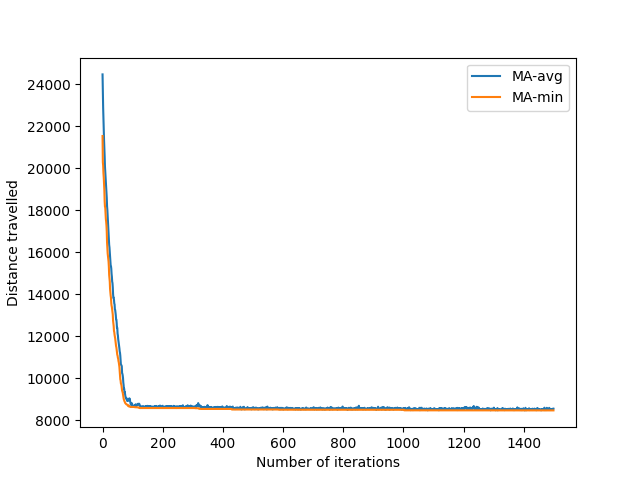
\includegraphics[width=0.5\textwidth]{6/6bMA_SYM}

\caption{Figures generated by TSPSolver. The higher and lower rows correspond to the TSPs in \texttt{file-tsp.txt} and \texttt{bays29.tsp} respectively, both found in the same directory as \texttt{TSPSolver.py}.\label{fig:6}}
\end{figure}



\section*{7}
\begin{itemize}
  \item[(a)]
    $T = \{x, y, z, \text{true}, \text{false}\}$. False isn't
    \emph{strictly} necessary, but otherwise it would be a trivial
    formula.

    $F = \{\land, \lor, \leftrightarrow\}$. These all have arity 2.

  \item[(b)]
    $T = \mathbb{R} \cup \{x, z\}$. Technically $0.234$ and $0.789$ are in
    $\mathbb{Q}$, so that would suffice, but taking the reals is more
    standard.

    $F = \{+, -, *\}$. These all have arity 2.

\end{itemize}

\section*{8}
See figure \ref{fig8}. We used the DEAP python framework. Any individuals with
errors (so, if it tried to divide by 0, or log -1) were given fitness
$-\infty$. For the implementation see \texttt{8/code.py}, and to generate
the plots simply run \texttt{8/plots.py}. (Both are found in the GitHub repository
linked at the start of this document.)

\begin{figure}[ht!]
  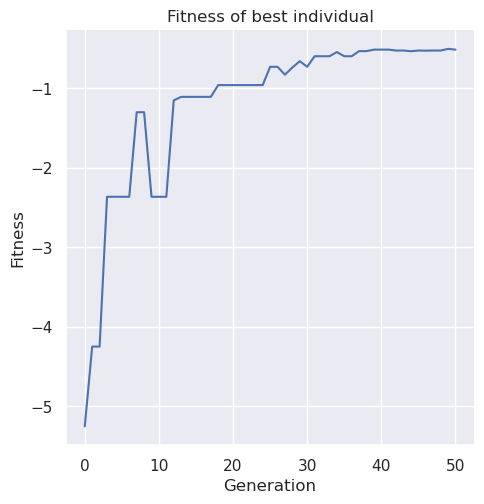
\includegraphics[width=0.5\textwidth]{8/score_best}
  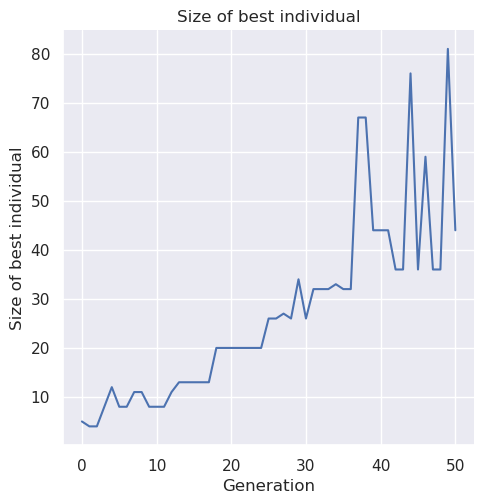
\includegraphics[width=0.5\textwidth]{8/size_best}
  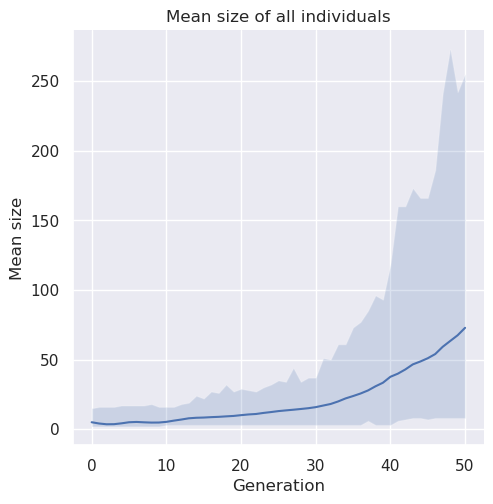
\includegraphics[width=0.5\textwidth]{8/mean_size}
  \caption{Exercise 8}
  \label{fig8}
\end{figure}

%TODO: maybe add a proper reference using a reference manager.
We do in fact see a undesirable phenomenon: bloat. Two techniques to
prevent this are given in the Javed, Noman, and Fermand Gobet paper, which
is also referenced in the lecture slides (page 47).

These techniques are generation-wide simplification (gws) and pruning. In
gws every $k$th generation (for some k) we simplify the trees. Instead of
producing offspring from mutation or crossover, we generate offspring by
selecting subtrees.

Pruning is a similar idea, but instead of doing it population-wide, we pick
the top few percent fittest individuals, and replace them by the fittest
out of some generated set of subtrees.

\end{document}
\end{document}
